\documentclass[conference]{IEEEtran}
\usepackage[T1]{fontenc}
\usepackage{amsmath}        % equation, align
\usepackage{graphicx}       % \includegraphics
\usepackage{booktabs}       % \toprule, \midrule, \bottomrule
\usepackage{tabularx}       % tables that fill the column
\usepackage{multirow}
\usepackage{algorithm}      % the floating box
\usepackage{algpseudocode}  % \State
\usepackage{hyperref}       % load last

% paper.tex lives in paper/, so ../ goes up to the project root. Figures are
% included as Sensor/figures/<name> or sim/figures/<name>, because the two
% runs use the same file names.
\graphicspath{{../outputs/}}

% Let floats share pages with text instead of each taking a page of its own.
\renewcommand{\topfraction}{0.9}
\renewcommand{\bottomfraction}{0.8}
\renewcommand{\textfraction}{0.1}
\renewcommand{\floatpagefraction}{0.8}
\renewcommand{\dbltopfraction}{0.9}
\renewcommand{\dblfloatpagefraction}{0.8}
\setcounter{topnumber}{3}
\setcounter{dbltopnumber}{2}
\setcounter{totalnumber}{4}

\title{On-Device Light-Source Classification with a\\1\,KB Density Lookup Table on an ESP32}
\author{\IEEEauthorblockN{Gib Macarine}
        \IEEEauthorblockA{Department of Computer Engineering\\
                          Vanier College}}

\begin{document}
\maketitle

\begin{abstract}
We deploy an unsupervised density classifier on an ESP32 and test it against real light sensors. Offline, DBSCAN discovers the lighting conditions in unlabelled UV and IR readings, a Gaussian kernel density estimate maps each one, and each map is stored as one byte per cell of a $16\times16$ grid. Online, a reading is classified with four byte reads and a reject threshold. On 2400 readings of shade, LED, fluorescent and sunlight, DBSCAN recovers the four conditions exactly against their true labels. The shipped model is 1040 bytes, held in flash with no SRAM cost, and a query takes 4.3\,\textmu s (12.7\,\textmu s median in the live loop). On 1344 fresh indoor readings recorded on the device, the ESP32 agrees with the desktop model on every decision and is correct on every one. Sunlight was not tested on the device. The EMA input filter preserves the class levels but does not suppress hand occlusions longer than about 0.3\,s.
\end{abstract}

%=====================================================================
\section{Proposed Pipeline}
%=====================================================================

The pipeline has two regimes. The \emph{offline} path runs once on a workstation. Both features are passed through $\log(1+x)$ and min--max scaled onto $[0,1]^2$ using the training range (Section~\ref{sec:transform}). DBSCAN groups the training points by density into $K$ classes and labels the rest noise. A Gaussian KDE is fitted to each class, normalised to its own peak, sampled onto a $G\times G$ grid and stored as \texttt{uint8}. A generator script writes the result to \texttt{model.h}: the $K$ byte tables, the four scaling bounds, the class names and $\tau$.

The \emph{online} path, Algorithm~\ref{alg:lookup}, runs on the ESP32. It contains no training data, no kernel evaluation and no distance loop, so its cost is $K$ byte reads and $K$ comparisons, regardless of how much data built the tables.

\begin{algorithm}[!bt]
\caption{ESP32 inference loop (online path).}
\label{alg:lookup}
\begin{algorithmic}[1]
\Require \texttt{model.h}: tables $Q_1,\dots,Q_K$ ($G\times G$ bytes), bounds $(x_{\min},x_{\max},y_{\min},y_{\max})$ in log units, threshold $\tau$; EMA factor $\alpha$
\State Read raw UV $x_n$ (ADC) and IR $y_n$ (TSL2591 IR channel). Filter both: $\bar{x}_n \gets \alpha x_n + (1-\alpha)\bar{x}_{n-1}$, likewise $\bar{y}_n$.
\State Transform and scale: $\tilde{x} \gets (\log(1+\bar{x}_n) - x_{\min})/(x_{\max}-x_{\min})$; likewise $\tilde{y}$ from $\bar{y}_n$, $y_{\min}$, $y_{\max}$.
\State Find the cell: $\text{col} \gets \lfloor \tilde{x}G \rfloor$, $\text{row} \gets \lfloor \tilde{y}G \rfloor$, each clipped to $[0, G-1]$.
\State Set the class counter $c \gets 1$, best class $\hat{c} \gets 1$, best value $v^{*} \gets -1$.
\State Read one byte: $v_c \gets Q_c[\text{row},\text{col}]/255$. If $v_c > v^{*}$, set $v^{*} \gets v_c$ and $\hat{c} \gets c$.
\State Increase $c$. If $c \le K$, repeat step 5; else go to step 7.
\State If $v^{*} < \tau$, report \textsc{unknown} and go to step 9.
\State Report class name $\hat{c}$.
\State Wait for the next sample (100\,ms), then go to step 1.
\end{algorithmic}
\end{algorithm}

Two details of Algorithm~\ref{alg:lookup} are deliberate. First, it uses nearest-cell lookup ($K$ reads) rather than bilinear blending ($4K$ reads); on the synthetic validation, both lookups gave the same decisions (Section~\ref{sec:sim}). Second, the reject test in step~7 is not optional. Without it, the algorithm returns a confident label everywhere, including regions no training reading ever reached. The strict comparison in step~5 keeps the lowest-numbered class on a tie, matching \texttt{numpy.argmax} on the desktop.

%=====================================================================
\section{Application}
%=====================================================================

The target is the always-on sensor hub of a phone or wearable: a small, low-power microcontroller that reads the ambient-light sensor while the main processor sleeps. Today such hubs estimate brightness for the display. Classifying the \emph{kind} of light (outdoors, LED, fluorescent, dim interior) would let the device pick a display profile, so that colour temperature and brightness adapt to the source as well as its level.

The pipeline fits this setting for three reasons. The flash budget is small and shared among many always-on features, and the model is 1040 bytes. Labels are expensive: individual sensor units read differently, and labelling calibration data for each unit is impractical, whereas clustering unlabelled readings can run per device. Finally, the classes are not round blobs. Sunlight readings stretch along a long streak as clouds pass, and indoor readings drift with distance, which suits a density method better than a centre-based one.

%=====================================================================
\section{Method and Setup}
%=====================================================================

\subsection{Hardware}
The prototype is an ESP32 DevKit (240\,MHz, 4\,MB flash) with two sensors (Fig.~\ref{fig:wiring}, Fig.~\ref{fig:photo}). UV is read from a GUVA-S12SD module (Octopus board) on GPIO34, an ADC1 pin, with 12-bit resolution. The IR channel deviates from the assignment's analog photodiode. The specified EPD-712 photodiode produced only millivolt-level signals through the 10\,k$\Omega$ divider under indoor light, which falls in the noisiest region of the ESP32's ADC; amplifying it would have required an additional transimpedance stage. On the instructor's recommendation, IR is instead read from a Waveshare TSL25911 (TSL2591) over I$^2$C. It integrates and digitises the photodiode current on-chip. Its IR-only channel is used, at medium gain and 100\,ms integration. The firmware reports each decision over serial and on one LED per class.

\begin{figure}[!t]
\centering
\includegraphics[width=\columnwidth]{Sensor/figures/wiring.pdf}
\caption{Prototype wiring. UV is read on GPIO34 (ADC1), IR over I$^2$C (SDA GPIO21, SCL GPIO22); both sensors run from 3.3\,V. GPIO32, 33, 25, 26 and 27 drive one LED per class plus \textsc{unknown}.}
\label{fig:wiring}
\end{figure}

\subsection{Data Collection and Filtering}
The collection firmware and the labelled dataset were forked from a peer's repository~\cite{peer_repo}. Readings are logged over USB serial as \texttt{sensor1,sensor2,label} rows at about 10\,Hz. Serial was chosen because the board is tethered to a laptop during collection anyway, and it needs no SD card or network code. The dataset has 600 rows for each of four conditions (shade, LED, fluorescent and direct sun), 2400 in all. The label column is removed before the pipeline sees the data and is used only for scoring.

Each raw reading is passed through an exponential moving average, $\bar{x}_n = \alpha x_n + (1-\alpha)\bar{x}_{n-1}$ with $\alpha = 0.2$, before it is logged or classified. An EMA costs one multiply-add and one stored value per channel, with no buffer, and $\alpha = 0.2$ gives a time constant of about five samples (0.5\,s). The same filter, constant and sample rate must run on the device, because the model was trained on its output. Section~\ref{sec:filter} tests how well it removes glitches.

\subsection{Feature Transform and Scaling}
\label{sec:transform}
Indoors, UV reads exactly 0, so shade, LED and fluorescent are separated by IR alone, while UV only distinguishes sun. IR spans 131 (shade) to about 31\,900 (sun). Scaled linearly, sun stretches the range so far that all three indoor classes fall inside the bottom 0.8\% of the axis, which is a single grid row (Fig.~\ref{fig:logscale}, left). There, no bandwidth or grid choice can separate them, and DBSCAN finds only two clusters at $\varepsilon = 0.03$ and $0.06$. Applying $\log(1+x)$ before min--max scaling spreads the indoor classes over the bottom 19\% of the axis, across four grid rows (Fig.~\ref{fig:logscale}, right). DBSCAN then finds the four classes at every $\varepsilon$ from 0.003 to 0.06. We use $\log(1+x)$ rather than $\log x$ because UV is exactly 0 indoors. The four scaling bounds are stored in log units, so the device applies the same transform first (Algorithm~\ref{alg:lookup}, step~2).

\begin{figure}[!t]
\centering
\includegraphics[width=\columnwidth]{Sensor/figures/log_vs_linear.pdf}
\caption{Scaled IR of the 1440 training readings by true condition, with the 16 grid rows marked. Left: linear scaling puts shade, LED and fluorescent in row~0. Right: $\log(1+x)$ separates them into rows 0--3.}
\label{fig:logscale}
\end{figure}

\subsection{Split, Clustering, Density Maps and Storage}
The 2400 readings are split once (seed 20250903) into training (1440), validation (480) and test (480) sets. DBSCAN runs on the scaled training points with $\varepsilon = 0.06$ and \texttt{min\_samples}~$=8$, and finds four clusters with no noise. For each cluster, a Gaussian KDE is fitted to its points and normalised to its own peak, so the largest class does not dominate close decisions. The bandwidth was chosen by mean log-likelihood on the validation set (Table~\ref{tab:bandwidth}). Each map is sampled at the centres of a $16\times16$ grid and stored as $q = \operatorname{round}(255\,g)$, so a stored value is off by at most $1/(2\cdot255) = 0.196\%$ of peak. The measured worst case over all cells is 0.187\%. The reject threshold is $\tau = 0.12$, about 31 of 255, set by hand. The model costs
\begin{equation}
    K \cdot G^2 + 16 = 4 \cdot 16^2 + 16 = 1040\ \text{bytes},
    \label{eq:flash}
\end{equation}
where the 16 bytes are the four \texttt{float32} bounds. The generator script writes it to \texttt{model.h} as a \texttt{const} array, which the ESP32 keeps in flash.

\begin{table}[!bt]
\centering
\caption{Bandwidth selection on the 480 validation readings. Each $h$ is fitted on training data only.}
\label{tab:bandwidth}
\small\setlength{\tabcolsep}{4pt}
\begin{tabular}{@{}l ccccccc@{}}
\toprule
$h$ & \textbf{0.03} & 0.04 & 0.05 & 0.06 & 0.08 & 0.10 & 0.12 \\
\midrule
Log-lik. & \textbf{5.16} & 4.66 & 4.31 & 4.04 & 3.61 & 3.27 & 2.98 \\
\bottomrule
\end{tabular}
\end{table}

%=====================================================================
\section{Evidence}
\label{sec:evidence}
%=====================================================================
Each result below is introduced by the claim it supports.

\subsection{The Method Was Validated First on Synthetic Data}
\label{sec:sim}
Before real sensors were used, the same pipeline was run on synthetic data where the correct answer is known: two crescents, a ring and uniform background noise, 1030 points in all. DBSCAN recovered the three shapes and labelled the background as noise. k-means, given $k=3$, has no noise label and assigned every background point to a shape (Fig.~\ref{fig:sim}). The ring's empty centre, surrounded by data but containing none, was answered \textsc{unknown}. The stored \texttt{uint8} model matched the continuous KDE on all 206 synthetic test points, and nearest-cell and bilinear lookup gave the same class. These results justify the design choices carried over to real data: a density method, a reject threshold, and byte storage.

\begin{figure}[!t]
\centering
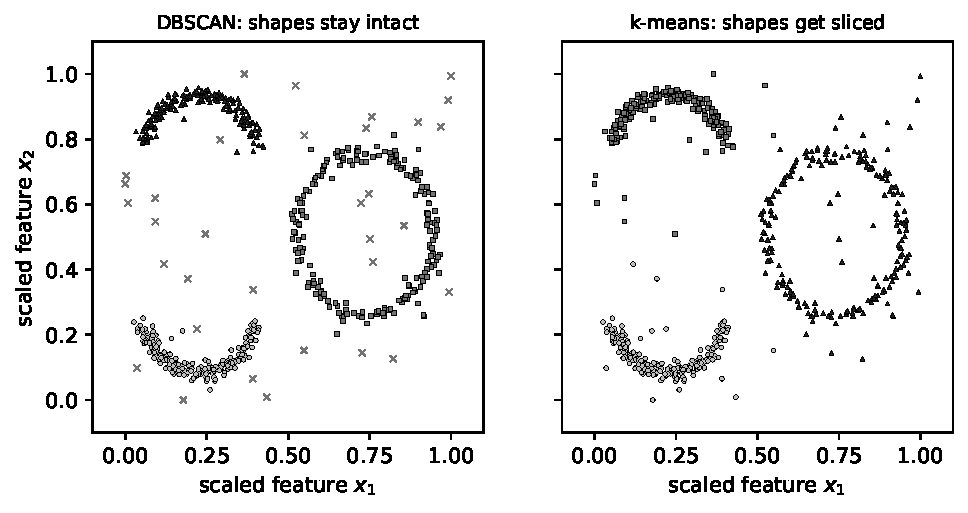
\includegraphics[width=\columnwidth]{sim/figures/clustered_space.pdf}
\caption{Synthetic validation, 618 training points. Left: DBSCAN keeps both crescents and the ring intact and marks background points as noise ($\times$). Right: k-means with $k=3$ assigns every point, noise included, to a centre.}
\label{fig:sim}
\end{figure}

\subsection{DBSCAN Recovers the True Lighting Conditions}
Table~\ref{tab:truth} scores the four discovered clusters against the labels that DBSCAN never saw. Every cluster is exactly one condition, and no reading is labelled noise. The agreement is complete because, after the log transform, the four conditions sit far apart compared with $\varepsilon$. The data were recorded in one session at a fixed distance, so this separation is easier than in field use (Section~\ref{sec:limits}).

\begin{table}[!bt]
\centering
\caption{DBSCAN clusters against true labels, 1440 training readings ($\varepsilon=0.06$, \texttt{min\_samples}~$=8$).}
\label{tab:truth}
\small
\begin{tabularx}{\linewidth}{@{}X rrrrr@{}}
\toprule
True label & c0 & c1 & c2 & c3 & noise \\
\midrule
shade       & \textbf{339} & 0 & 0 & 0 & 0 \\
sun         & 0 & \textbf{354} & 0 & 0 & 0 \\
fluorescent & 0 & 0 & \textbf{371} & 0 & 0 \\
LED         & 0 & 0 & 0 & \textbf{376} & 0 \\
\bottomrule
\end{tabularx}
\end{table}

\subsection{The Stored Model Is a Faithful Copy}
Fig.~\ref{fig:stored} shows the complete shipped model. The four classes occupy five of the 256 cells: shade, LED and fluorescent sit in column~0, because UV is 0 indoors, and sun in the far corner. The other 251 cells (98\%) are below $\tau$. A reading between indoor light and sun, such as raw (1000, 2000), is answered \textsc{unknown}. On the 480 held-out test readings, the stored \texttt{uint8} lookup and the continuous KDE gave the same decision for all 480.

\begin{figure*}[!t]
\centering
\includegraphics[width=0.85\textwidth]{Sensor/figures/class_surfaces_discretized.pdf}
\caption{The shipped model: one $16\times16$ \texttt{uint8} table per class, 1024 bytes in total. Classes 0--3 are shade, sun, fluorescent and LED. The three indoor classes sit in column~0 (UV $=0$), separated only by IR row.}
\label{fig:stored}
\end{figure*}

\subsection{The Filter Keeps Class Levels but Not Long Glitches}
\label{sec:filter}
Fig.~\ref{fig:filter} records 22\,s of raw and filtered IR under fluorescent light while a hand was passed over the sensor seven times. Each pass dropped the raw reading for 3 to 10 samples (0.3--1\,s). Between passes, the EMA settles to the same level as the raw signal, so it does not erase the difference between classes: fluorescent stays well inside its band. It does not remove occlusions of this length, though. It spreads each dip over about 0.5\,s, and because LED and shade lie between fluorescent and darkness on the IR axis, the output passes through both on the way down and back. Of the 222 samples, all truly fluorescent, the unfiltered signal would be misclassified 36 times and the EMA output 44 times. Seventeen of those 44 occur after the raw reading has already recovered. Replaying the capture offline, adding an output hold (report a new class only after it appears five times in a row) on top of the same EMA reduces this to 11, without changing the model.

\begin{figure}[!t]
\centering
\includegraphics[width=\columnwidth]{Sensor/figures/raw_vs_filtered.pdf}
\caption{Raw and EMA-filtered IR under fluorescent light, with seven hand passes over the sensor. Dashed lines are the grid-row boundaries between classes. The strip shows the class the device reported.}
\label{fig:filter}
\end{figure}

\subsection{The Device Agrees with the Desktop on Fresh Data}
A fresh batch was recorded on the device under each indoor condition (Table~\ref{tab:heldout}). For each reading, the ESP32 logged the filtered values, its decision and the true label. All 1344 decisions were correct, and replaying the logged values through the Python pipeline reproduced every one: on-device and desktop agreement is 100\%. The LED and fluorescent batches spread wider than the training data (IR 197--242 against 224--229 for LED), yet stayed in their cells. Indoors, a class's cell spans a band of IR values (LED: about 185--262), so the coarse grid tolerates this drift.

\begin{table}[!bt]
\centering
\caption{Fresh held-out batch recorded on the ESP32.}
\label{tab:heldout}
\small\setlength{\tabcolsep}{4pt}
\begin{tabularx}{\linewidth}{@{}X r c c r@{}}
\toprule
Condition & Rows & IR, fresh & IR, train & Correct \\
\midrule
shade       & 440 & 133--142 & 131--153 & 440 \\
LED         & 464 & 197--242 & 224--229 & 464 \\
fluorescent & 440 & 342--370 & 360--383 & 440 \\
sun         & --- & \multicolumn{2}{c}{not tested on device} & --- \\
\midrule
Total       & 1344 & & & 1344 \\
\bottomrule
\end{tabularx}
\end{table}

\subsection{Measured Cost Matches the Prediction}
Table~\ref{tab:cost} compares the firmware's own measurements with \eqref{eq:flash}. The model size matches exactly, and its table address lies in the ESP32's flash-mapped data region, so it costs no SRAM. The whole sketch is 332\,800 bytes, of which the model is 0.3\%. The rest is the Arduino core and sensor libraries. A query takes 4.28\,\textmu s averaged over 10\,000 back-to-back calls, and a median of 12.65\,\textmu s in the live loop. The difference is cache behaviour: between live queries, the I$^2$C read evicts the classifier and table from the flash cache. Most of each query is the two $\log(1+x)$ calls and the divisions, not the four byte reads. Either figure is under 0.02\% of the 100\,ms sample period.

\begin{table}[!bt]
\centering
\caption{Predicted against measured cost on the ESP32 (240\,MHz).}
\label{tab:cost}
\begin{tabularx}{\linewidth}{@{}X r r@{}}
\toprule
Quantity & Predicted & Measured \\
\midrule
Model (tables + bounds) & 1040\,B & 1040\,B \\
Model SRAM             & 0\,B    & 0\,B (in flash) \\
Sketch flash           & ---     & 332\,800\,B \\
Heap in use            & ---     & 43\,572\,B \\
Query, back-to-back    & few \textmu s & 4.28\,\textmu s \\
Query, live (median)   & ---     & 12.65\,\textmu s \\
\bottomrule
\end{tabularx}
\end{table}

\subsection{Proof of Concept}
Fig.~\ref{fig:photo} shows the prototype. A video of live classification is available at \url{https://youtu.be/epPjHrj3CWY}.

\begin{figure}[!t]
\centering
\includegraphics[width=0.8\columnwidth]{Sensor/figures/board_photo.jpg}
\caption{The prototype: ESP32 DevKit on the breadboard, the GUVA-S12SD UV board (top right) and the TSL25911 IR sensor (bottom).}
\label{fig:photo}
\end{figure}

%=====================================================================
\section{Limitations and Remaining Uncertainty}
\label{sec:limits}
%=====================================================================

\textbf{Sunlight was not tested on the device.} During testing, the UV board read 0 outdoors in late-afternoon sun, which is consistent with near-zero UV at a low sun angle but does not rule out a fault. Sun is therefore validated only on the desktop test split. Since the GUVA-S12SD board differs from the one used to collect the training data, its gain may differ as well.

\textbf{The training data come from one session and one place.} Agreement with true labels and with the device was measured under the same lights at the same distance. A first device recording in a different spot read shade at IR 96--107, below the training minimum of 131, and was excluded from the held-out batch. Readings below the training range are clipped into the edge cell, so darker-than-trained shade, or a covered sensor, is reported as shade, never \textsc{unknown}. The reject test only guards the interior of the grid.

\textbf{The filter does not suppress hand occlusions.} At $\alpha = 0.2$, the EMA is too slow to hide occlusions of 0.3\,s or more, and its lag sends the output through intermediate classes (Section~\ref{sec:filter}). An output hold reduced errors from 44 to 11 offline but is not yet in the firmware.

\textbf{The indoor classes rest on one feature.} UV is 0 for shade, LED and fluorescent, so they are separated only by IR level, by fixed boundaries at about 185 and 262 counts. A brighter LED or a closer lamp could cross a boundary and change class.

\textbf{Several settings are at an edge or set by hand.} Validation selected the smallest bandwidth in the sweep, so the optimum may be lower still, although a cell is already 1/16 wide. The threshold $\tau$ was not tuned. Sun IR reaches 87\% of the TSL2591's 36\,863-count ceiling at this gain, and sun UV is near the ADC's 4095 limit, so brighter conditions could saturate either sensor.

%=====================================================================
\section*{Acknowledgment}
%=====================================================================
The sensor hardware program (the TSL25911 and GUVA-S12SD data-collection firmware, including its EMA filter and sensor settings) and the labelled sensor dataset used in this work were forked from Gianluca D'Altorio's \texttt{data-collection} repository~\cite{peer_repo}. The DBSCAN, KDE and byte-table pipeline, the model generator and the inference firmware are the author's own, built on the course's Lab~3 code.

%=====================================================================
% References
%=====================================================================
\begin{thebibliography}{1}
\bibitem{peer_repo}
G. D'Altorio, ``data-collection,'' GitHub repository, 2026. [Online]. Available: \url{https://github.com/GianlucaDAltorio/data-collection}
\end{thebibliography}

\end{document}